\documentclass[12pt]{report}
\usepackage{commands}
\usepackage{matlab-prettifier}

\begin{document}

\large
\begin{center}
AMSC 660 Homework 9\\
Due 11/3\\
By Marvyn Bailly\\
\end{center}
\normalsize
\hrule

%Good luck my man

%---------------%
%---Problem 1---%
%---------------%


\begin{problem}%[vskip]
\subsection*{Problem 1}

Suppose that a smooth function $f(x)$ is approximated by a quadratic model in the neighborhood of a current iterate $x$:
\[
     m(p) = f(x) + \nabla f(x)^\top p + \frac{1}{2}p^\top Bp,
\]
where $B$ is a symmetric positive definite matrix. Show that then the direction $p$ found by setting the gradient of $m(p)$ to zero is the descent direction for $f(x)$, i.e.,
\[
     \cos(\theta) := - \frac{\nabla f(x)^\top p}{\|\nabla f(x)\|\|p\|}>0.
\]
Also, bound $\cos(\theta)$ away from zero in terms of the condition number of $B$, i.e. $\kappa(B) = \|B\|\|B^{-1}\|.$

\subsection*{Solution}
\begin{proof}
Suppose that a smooth function $f(x)$ is approximated by a quadratic model in the neighborhood of a current iterate $x$:
\[
        m(p) = f(x) + \nabla f(x)^\top p + \frac{1}{2}p^\top Bp,
\]
where $B$ is a symmetric positive definite matrix. Taking the gradient we get
\[
     \nabla m(p) = \nabla f(x)+ Bp,
\]
and setting $\nabla m(p) = 0$ we get
\[
     0 = \nabla f(x)+ Bp \implies = \nabla f(x) = -Bp.
\]
Plugging this into the descent direction we get
\begin{align*}
    \cos(\theta) &= \frac{-\nabla f(x)^\top p}{\|\nabla f(x)\|\|p\|} =\frac{(Bp)^\top p}{\|-Bp\|\|p\|}= \frac{p^\top B p}{\|-Bp\|\|p\|},\\
\end{align*}
and since $\|p\|^2 \leq \|B^{-1}\|p^\top Bp$, we get
\[
    \cos(\theta) \geq \frac{\|p\|^2}{\|B^{-1}\|\|B\|\|p\|^2} = \frac{1}{\|B^{-1}\|\|B\|} = \frac{1}{\kappa(B)}.
\]
Since we have that $B$ is SPD, we know that $\|B^{-1}\|\|B\| > 0$, therefore
\[
     \cos(\theta) > 0.
\]


\end{proof}
\end{problem}




%---------------%
%---Problem 2---%
%---------------%


\begin{problem}%[vskip]
\subsection*{Problem 2}

Let $f(x), x \in \R^n$, be a smooth arbitrary function. The BFGS method is a quasi-Newton method with the Hessian approximate built recursively by
\[
     B_{k+1} = B_k - \frac{B_ks_ks_k^\top B_k}{s_k^\top B_k s_k} + \frac{y_k y_k^\top}{y_k^\top s_k}, ~\text{where}~ s_k := x_{k+1} - x_k, ~y_k := \nabla f_{k+1} - \nabla f_k.
\]
Let $x_0$ be the starting point and let the initial approximation for the Hessian is the identity matrix.
\begin{enumerate}
    \item [(a)] Let $p_k$ be a descent direction. Show that Wolfe's condition 2,
    \[
         \nabla f_{k+1}^\top p_k \geq c_2 \nabla f_k^\top p_k, ~c_2 \in (0,1),
    \]
    implies that $y_k^\top s_k > 0$.


    \item [(b)] Let $B_k$ be symmetric positive definite. Prove that then $B_{k+1}$ is also SPD, i.e., for any $z \in \R^n\setminus {0}, z^\top B_{k+1}z>0$. You can use the previous item of this Problem and the Cauchy-Schwarz inequality for the $B_k$-inner product $(u,v)_{B_k} := v^\top B_k u$. 
    

\end{enumerate}

\def\n{{\nabla}}

\subsection*{Solution}
\begin{proof}

Let $f(x), x \in \R^n$, be a smooth arbitrary function. The BFGS method is a quasi-Newton method with the Hessian approximate built recursively by
\[
        B_{k+1} = B_k - \frac{B_ks_ks_k^\top B_k}{s_k^\top B_k s_k} + \frac{y_k y_k^\top}{y_k^\top s_k}, ~\text{where}~ s_k := x_{k+1} - x_k, ~y_k := \nabla f_{k+1} - \nabla f_k.
\]
Let $x_0$ be the starting point and let the initial approximation for the Hessian is the identity matrix.

\begin{enumerate}
    \item [(a)]
    Let $p_k$ be a descent direction. Observe that
    \begin{align*}
        y_k^\top s_k &= ( \n f_{k+1} - \n f_k)^\top(x_{k+1} - x_k)\\
        &= (\n f_{k+1} - \n f_k)^\top (\alpha_k p_k)\\
        &= \alpha_k(\n f_{k+1}^\top p_k - \n f_k^\top p_k)\\
        &\geq  \alpha_k(c_2\n f_{k}^\top p_k - \n f_k^\top p_k),
    \end{align*}
    by Wolfe's second condition where $c_2 \in (0,1)$. Now rewriting the terms we see that
    \[
        y_k^\top s_k \geq \alpha_k(c_2 -1)(\n f_{k}^\top p_k) \geq 0,
    \]
    since $\alpha_k > 0, (c_2 - 1) \leq 0$, and $\n f_{k}^\top p_k \leq 0$. 

    \item [(b)]
    Let $B_k$ be a symmetric positive definite. We wish to show that $B_{k+1}$ is also SPD. Let $z \in R^n \setminus 0$. Then observe that
    \begin{align*}
        z^\top B_{k+1} z &= z^\top \paren{B_k - \frac{B_ks_ks_k^\top B_k}{s_k^\top B_k s_k} + \frac{y_k y_k^\top}{y_k^\top s_k}} z\\
        &= z^\top B_k z - z^\top \frac{B_ks_ks_k^\top B_k}{s_k^\top B_k s_k}z + z^\top \frac{y_k y_k^\top}{y_k^\top s_k} z\\
        &= \abrac{z,z}_{B_k} - \frac{\abrac{z,s_k}_{B_k}^2}{\abrac{s_k,s_k}_{B_k}}  + \frac{\abrac{z,y_k}^2}{y_k^\top s_k}  \\
        &\geq  \abrac{z,z}_{B_k}  - \frac{\abrac{z,z}_{B_k}\abrac{s_k,s_k}_{B_k}}{\abrac{s_k,s_k}_{B_k}} + \frac{\abrac{z,y_k}^2}{y_k^\top s_k} \quad (\text{by Cauchy-Schwarz})\\
        &= \abrac{z,z}_{B_k} - \abrac{z,z}_{B_k} + \frac{\abrac{z,y_k}^2}{y_k^\top s_k}\\
        &= \frac{\abrac{z,y_k}^2}{y_k^\top s_k},
    \end{align*}
    and since $y_k^\top s_k > 0$ by the previous part, we have that $z^\top B_{k+1} z > 0$. 

\end{enumerate}





\end{proof}
\end{problem}





%---------------%
%---Problem 3---%
%---------------%

\begin{problem}%[vskip]
\subsection*{Problem 3}

The goal of this problem is to code, test, and compare various optimization
techniques on the problem of finding local minima of the potential energy function
of the cluster of $7$ atoms interacting according to the Lennard-Jones pair potential (for brevity, this cluster is denoted by LJ$_7$):
\[
     f = 4 \sum_{i=2}^7\sum_{j=1}^i(r_{ij}^{-12}-r_{ij}^{-6}), r_{ij} := \sqrt{(x_i - x_j)^2 +(y_i - y_j)^2 + (z_i - z_j)^2}.
\]
Note that it is recommended to reset the matrix Bk in the BFGS method to identity every $m$ steps. Try $m = 5$ and $m = 20$. Compare the performance of the five algorithms, the three algorithms above, steepest descent, and Newton's (already encoded) in terms of the number of iterations required to achieve convergence and by plotting the graph of $f$ and $\|\nabla f\|$ against the iteration number for each test case. Do it for each of the four initial conditions approximating the four local minima and ten random initial conditions.

\subsection*{Solution}
\begin{proof}
    


    \begin{table}[h!]
        \centering
        \begin{tabular}{l l l}
        method & iter count& min found \\
        \hline
        SD & 500.0000 & -15.5932 \\
        Newton & 210.0000 & -15.5932 \\
        BFGS & 79.0000 & -15.5932 \\
        FRCG & 173.0000 & -15.5932 \\
        PRCG & 248.0000 & -15.5932 \\
        \hline
        SD & 500.0000 & -15.5331 \\
        Newton & 87.0000 & -15.5331 \\
        BFGS & 60.0000 & -15.5932 \\
        FRCG & 129.0000 & -15.5331 \\
        PRCG & 185.0000 & -15.5331 \\
        \hline
        SD & 500.0000 & -15.5932 \\
        Newton & 109.0000 & -15.5932 \\
        BFGS & 66.0000 & -15.5932 \\
        FRCG & 135.0000 & -15.5932 \\
        PRCG & 215.0000 & -15.5932 \\
        \hline
        SD & 500.0000 & -13.4856 \\
        Newton & 500.0000 & -13.4856 \\
        BFGS & 105.0000 & -15.5331 \\
        FRCG & 275.0000 & -15.9350 \\
        PRCG & 312.0000 & -15.5331 \\
        \hline
        SD & 500.0000 & -15.5331 \\
        Newton & 118.0000 & -15.5331 \\
        BFGS & 79.0000 & -16.5054 \\
        FRCG & 140.0000 & -15.5331 \\
        PRCG & 239.0000 & -15.5331 \\
        \hline
        \end{tabular}
        \quad % Space between the two columns of the table
        \begin{tabular}{l l l}
        method & iter count& min found \\
        \hline
        SD & 500.0000 & -15.3853 \\
        Newton & 500.0000 & -15.5331 \\
        BFGS & 85.0000 & -15.5331 \\
        FRCG & 183.0000 & -15.5331 \\
        PRCG & 206.0000 & -15.5331 \\
        \hline
        SD & 466.0000 & -16.5054 \\
        Newton & 216.0000 & -16.5054 \\
        BFGS & 80.0000 & -16.5054 \\
        FRCG & 149.0000 & -16.5054 \\
        PRCG & 189.0000 & -16.5054 \\
        \hline
        SD & 500.0000 & -15.5331 \\
        Newton & 150.0000 & -15.5331 \\
        BFGS & 59.0000 & -15.5331 \\
        FRCG & 124.0000 & -15.5331 \\
        PRCG & 213.0000 & -15.5331 \\
        \hline
        SD & 500.0000 & -16.4884 \\
        Newton & 132.0000 & -16.5054 \\
        BFGS & 79.0000 & -16.5054 \\
        FRCG & 188.0000 & -16.5054 \\
        PRCG & 206.0000 & -16.5054 \\
        \hline
        SD & 500.0000 & -15.5328 \\
        Newton & 314.0000 & -15.5331 \\
        BFGS & 157.0000 & -15.5331 \\
        FRCG & 260.0000 & -15.5331 \\
        PRCG & 500.0000 & -15.5331 \\
        \hline
        \end{tabular}
        \caption{Results of the five algorithms ran on random initial conditions.}
        \label{table:lots of data}
        \end{table}
        
        \begin{figure}[H]
            \begin{subfigure}[b]{0.5\linewidth}
                \centering
                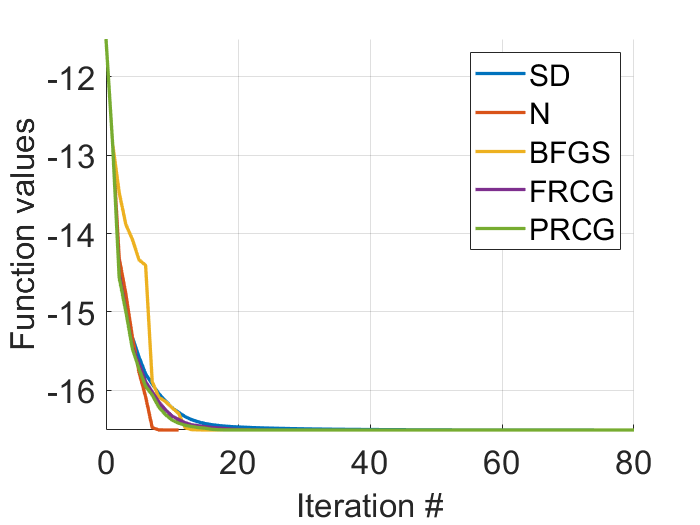
\includegraphics[width=\linewidth]{images/1-funcval.png}
                \caption{}
                \label{fig1:a}
                \vspace{4ex}
            \end{subfigure}%%
            \begin{subfigure}[b]{0.5\linewidth}
                \centering
                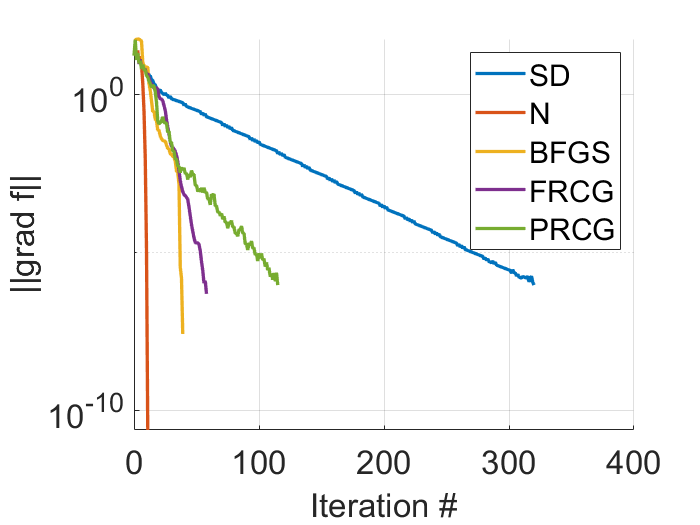
\includegraphics[width=\linewidth]{images/1-gradf.png}
                \caption{}
                \label{fig1:b}
                \vspace{4ex}
            \end{subfigure}
            \caption{Function values of the five methods at each iteration are shown in (a) while the norm of the norm of the gradient of the function value is shown in (b) when starting at the first initial condition.}
            \label{fig1}
        \end{figure}

        \begin{figure}[H]
            \begin{subfigure}[b]{0.5\linewidth}
                \centering
                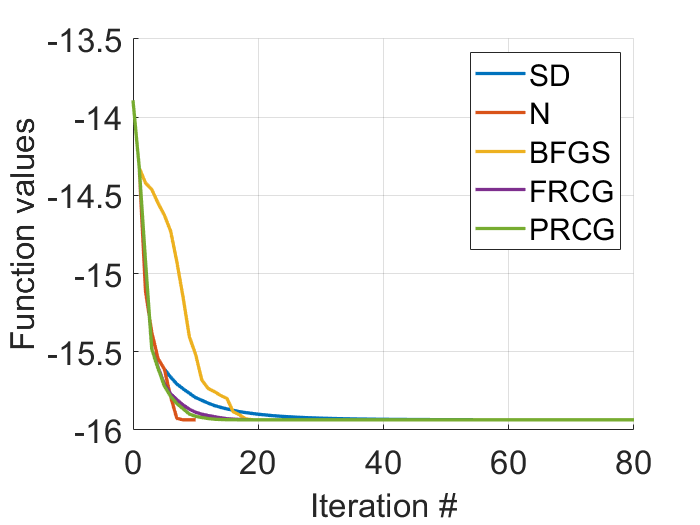
\includegraphics[width=\linewidth]{images/2-funcval.png}
                \caption{}
                \label{fig2:a}
                \vspace{4ex}
            \end{subfigure}%%
            \begin{subfigure}[b]{0.5\linewidth}
                \centering
                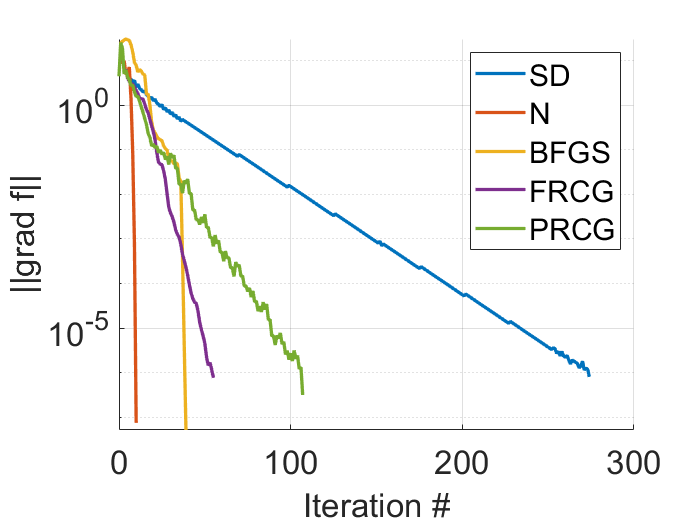
\includegraphics[width=\linewidth]{images/2-gradf.png}
                \caption{}
                \label{fig2:b}
                \vspace{4ex}
            \end{subfigure}
            \caption{Function values of the five methods at each iteration are shown in (a) while the norm of the norm of the gradient of the function value is shown in (b) when starting at the second initial condition.}
            \label{fig2}
        \end{figure}
        \begin{figure}[H]
            \begin{subfigure}[b]{0.5\linewidth}
                \centering
                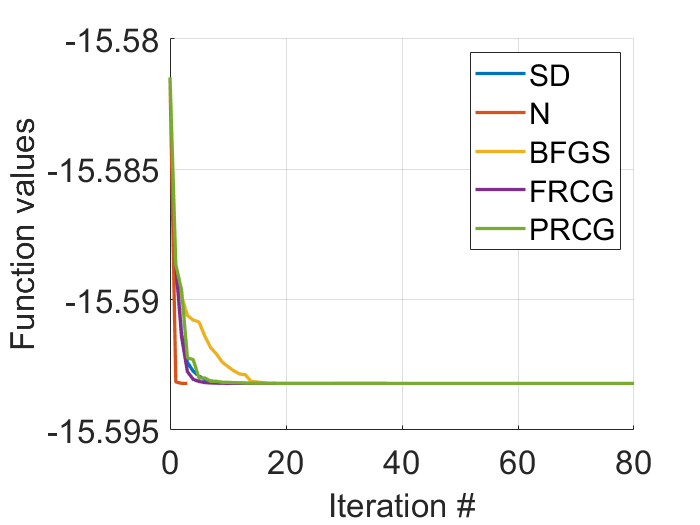
\includegraphics[width=\linewidth]{images/3-funcval.png}
                \caption{}
                \label{fig3:a}
                \vspace{4ex}
            \end{subfigure}%%
            \begin{subfigure}[b]{0.5\linewidth}
                \centering
                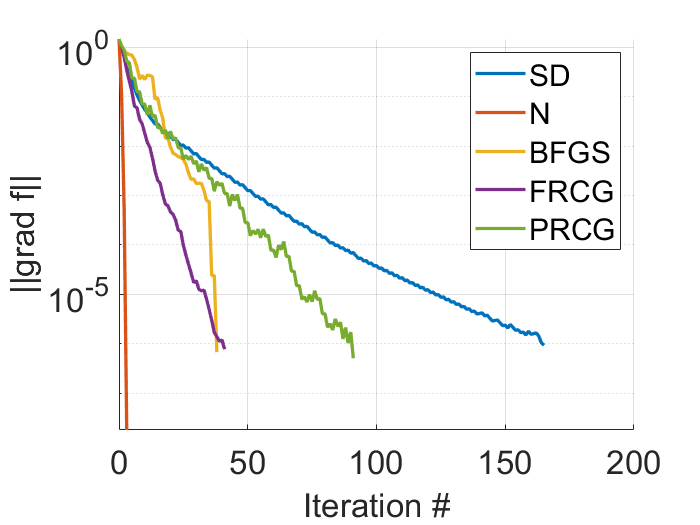
\includegraphics[width=\linewidth]{images/3-gradf.png}
                \caption{}
                \label{fig3:b}
                \vspace{4ex}
            \end{subfigure}
            \caption{Function values of the five methods at each iteration are shown in (a) while the norm of the norm of the gradient of the function value is shown in (b) when starting at the third initial condition.}
            \label{fig3}
        \end{figure}
        \begin{figure}[H]
            \begin{subfigure}[b]{0.5\linewidth}
                \centering
                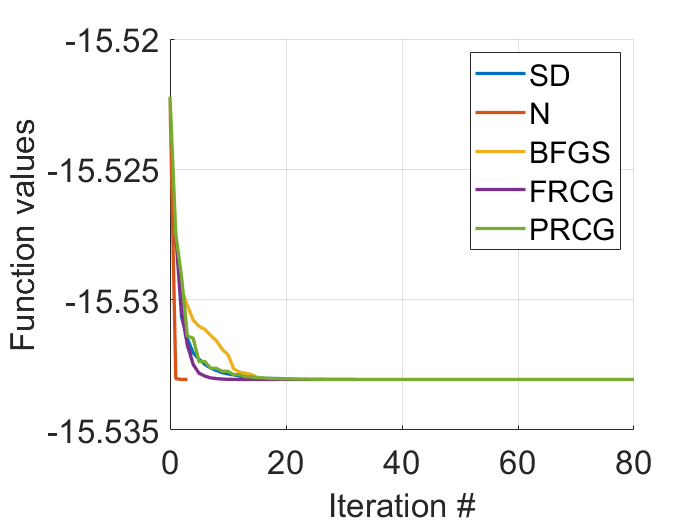
\includegraphics[width=\linewidth]{images/4-funcval.png}
                \caption{}
                \label{fig4:a}
                \vspace{4ex}
            \end{subfigure}%%
            \begin{subfigure}[b]{0.5\linewidth}
                \centering
                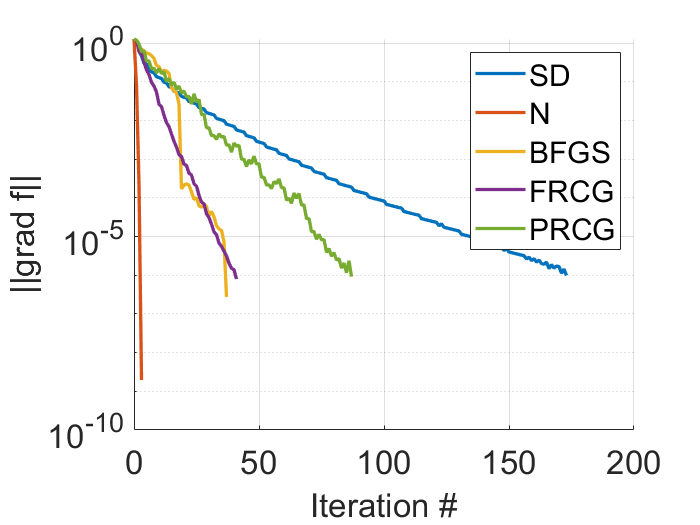
\includegraphics[width=\linewidth]{images/4-gradf.png}
                \caption{}
                \label{fig4:b}
                \vspace{4ex}
            \end{subfigure}
            \caption{Function values of the five methods at each iteration are shown in (a) while the norm of the norm of the gradient of the function value is shown in (b) when starting at the fourth initial condition.}
            \label{fig4}
        \end{figure}
        \begin{figure}[H]
            \begin{subfigure}[b]{0.5\linewidth}
                \centering
                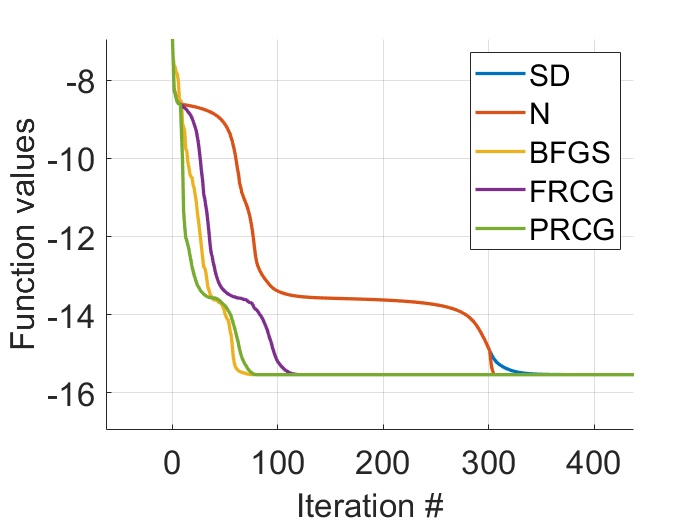
\includegraphics[width=\linewidth]{images/random-funcval.png}
                \caption{}
                \label{figRandom:a}
                \vspace{4ex}
            \end{subfigure}%%
            \begin{subfigure}[b]{0.5\linewidth}
                \centering
                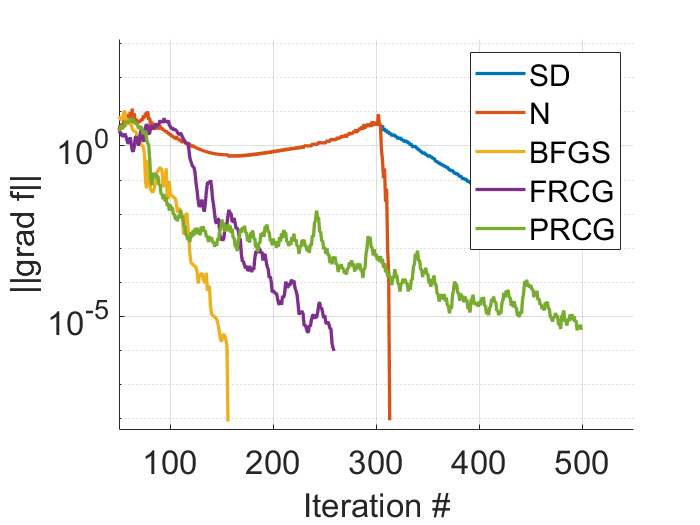
\includegraphics[width=\linewidth]{images/random-gradf.png}
                \caption{}
                \label{figRandom:b}
                \vspace{4ex}
            \end{subfigure}
            \caption{Function values of the five methods at each iteration are shown in (a) while the norm of the norm of the gradient of the function value is shown in (b) when starting at a random initial condition.}
            \label{figRandom}
        \end{figure}

        
        We begin by implementing the BFGS algorithm into the MATLAB code with the following:
        \begin{lstlisting}[style=Matlab-editor]
case 3 % BFGS
    if iter == 1
        p = -B\g;
    else
        s = x - xtemp;
        y = g - gtemp;
        if(mod(iter,BFGSReset)==0)
            B = eye(length(x),length(x));
        else
            B = B - (B*s*s'*B)/(s'*B*s) + (y*y')/(y'*s);
        end
        p = -B\g;
    end
    dir = "BFGS";
        \end{lstlisting}
        where \verb+xtemp+ and \verb+gtemp+ correspond to $x_{k-1}$ and $\nabla f_(x_{k-1})$. We use the variable \verb+BFGSReset+ to reset the $B$ matrix after a certain amount of iterations to the identity matrix. We found the best results when using $m=20$. Next, we implement the Fletcher-Reeves nonlinear CG (FRCG) algorithm as
        \begin{lstlisting}[style=Matlab-editor]
case 4 % Fletcher-Reeves nonlinear CG
    if iter == 1
        p = - g;
    else 
        beta = (g'*g)/(gtemp'*gtemp);
        p = -g + beta *p;
    end 
    dir = "FRCG";
        \end{lstlisting}
        Next, we implement the Polak-Ribiere nonlinear CG method (PRCG) algorithm as 
        \begin{lstlisting}[style=Matlab-editor]
case 5 % Polak-Ribiere nonlinear CG
    if iter == 1
        p = -g;
    else
        beta = (g'*(g-gtemp))/norm(gtemp)^2;
        beta = max(beta,0);
        p = -g + beta*p;
    end
    dir = "PRCG";
        \end{lstlisting}
        To compare the performance of the five algorithms, we needed to find a reasonable \verb+c+ value that worked for all five algorithms. Upon multiple tests, we concluded that $c = 0.25$ was an okay choice. We used two stopping conditions, the first being a max iteration count of $500$ and the second being the norm of the gradient of $f$ being less than $10^{-6}$. Next, we ran five algorithms for the four initial conditions approximating the four local minima and plotting the function value and $\|\nabla f\|$ against the iteration numbers as seen in Figure \ref{fig1}, Figure \ref{fig2}, Figure \ref{fig3}, and Figure \ref{fig4} for the four respective local minima. We see that for all four methods, the Newton method converges to the minima the fastest which corresponds with what we expect. We see that the BFGS and FRCG converge in a similar amount of iterations while the PRCG takes almost double. Finally, we have that the SD method takes the longest and usually either hits the max iteration count or the max tolerance. Running the five methods on ten different random initial conditions, one random initial condition is shown in Figure \ref{figRandom} and the results of all ten are summarized in Table \ref{table:lots of data}, we see that the BFGS method consistently converges the fastest and almost always finds the correct minima (in one case there appears to be rounding error). We note that the SD method always hits the max iteration count and doesn't always achieve the minima as a result. This also means that in some cases the Newton method also hits the max iteration count if the Hessian matrix isn't SPD. But once the matrix is SPD, the Newton method converges rapidly as seen in the first four examples. It appears that the FRCG method converges slowly than the BFGS method but more rapidly than the PRCG method.

        The code made for this method can be found at \url{https://github.com/MarvynBailly/AMSC660/tree/main/homework9}.
\end{proof}
\end{problem}

%---------------%
%---Problem 4---%
%---------------%


\begin{problem}%[vskip]
\subsection*{Problem 4}

\begin{enumerate}
    \item [(a)] Compute the gradient and the Hessian of the Rosenbrock function
    \[
         f(x,y) = 100(y - x^2)^2 + (1-x)^2.
    \]
    Show that $(1,1)$ is the only local minimizer, and that the Hessian is positive definite at it.
    \item [(b)] Program the steepest descent, FRCG, PRCG, Newton's, and BFGS algorithms using the backtracking line search Use them to minimize the Rosenbrock function. First start with the initial guess $(1.2, 1.2)$ and then with the more difficult one $(-1.2, 1)$. Set the initial step length $\alpha_0 = 1$ and plot the step length $\alpha_k$ versus $k$ for each of the methods. Plot the level sets of the Rosenbrock function using the command contour and plot the iterations for each methods over it. Plot $\|(x_k,y_k) - (x^*,y^*)\|$ versus $k$ in the logarithmic scale along the $y$-axis for each method. Do you observe a superlinear convergence? Compare the performance of the methods.
\end{enumerate}

\subsection*{Solution}
\begin{proof}

    \item [(a)] Consider Rosenbrock function
    \[
         f(x,y) = 100(y - x^2)^2 + (1-x)^2.
    \]
    Notice that the gradient is given by
    \[
         \nabla f(x,y) = (400x^3 -400xy + 2x - 2,200y-200x^2),
    \]
    and the Hessian is given by
    \[
        \mathbf{H}_f = \begin{pmatrix}
            2 + 800 x^2 - 400 (y - x^2) & -400 x \\
            -400 x & 200
        \end{pmatrix}.
    \]
    To show that $(1,1)$ is the only local minimizer, observe that
    \[
        \nabla f = 0 \implies \begin{cases}
            -400xy +400x^3 - 2+2x = 0\\
            200y - 200x^2 = 0,
        \end{cases}
    \]
    so $x^2=y$ and thus
    \[
        -400x^3 +400x^3 - 2+2x = 0 \implies x = 1,
    \]
    so $y = 1$. Thus we have that the only local minimizer of the Rosenbrock function is $(x,y) = (1,1)$. Notice that
    \[
         \mathbf{H}_f(1,1) = \begin{pmatrix}
            802 & -400 \\
            -400 & 200
        \end{pmatrix},
    \]
    which has eigenvalues $\lambda = 501 \pm \sqrt{250601} > 0$ and thus $\mathbf{H}_f(1,1)$ is positive definite since its eigenvalues are greater than zero.
    \item[(b)]
    The code made for this method can be found at \url{https://github.com/MarvynBailly/AMSC660/tree/main/homework9}. 
    
    To compare the four methods, we found a common \verb+c+ value of $c=0.45$ that worked reasonably for all the methods. We started with an initial guess of $(1.2,1.2)$ and the n changed to a more difficult one of $(-1.2,1)$ \footnote{We omit the graphs for the $(1.2,1.2)$ case.}. Using an initial step length of $\alpha_0 = 1$, a max iteration of $500$ and tolerance on the norm of $10^{-9}$, we get the following graphs: in Figures \ref{fig4-1},\ref{fig4-2},\ref{fig4-3},\ref{fig4-4} we see the $\alpha_k$ step size compared to the iteration and the iterate function value plotted on the contour of the Rosenbrock function for the steepest descent, Newton, BFGS, FRCG, and PRCG methods respectively. We see that all the methods are able to find the minimum of the function except for the steepest descent since the algorithm hits the maximum iterations. Next, we plot $\|(x_k,y_k) - (x^*,y^*)\|$ versus $k$ in the logarithmic scale along the $y$-axis for each method. The result can be seen in Figure \ref{fig4-6} where we see that Newton's method converges the fastest closely followed by BFGS. I would think that if we started at a further away initial condition or a more difficult function, BFGS may beat Newton. Slower than BFGS we see that PRCG beats FRCG and all methods are significantly faster than the SD method. By plotting a linear convergence line from the origin, we see that both Newton and BFGS converge faster than it, suggesting that both methods converge superlinearly. On the other hand, FRCG, PRCG, and SD methods converge slower than linear. If we plot a comparison linear line of convergence near the point where FRCG and PRCG began to rapidly converge, it also appears that they converge either linearly or near superlinearly.   

        \begin{figure}[H]
            \begin{subfigure}[b]{0.5\linewidth}
                \centering
                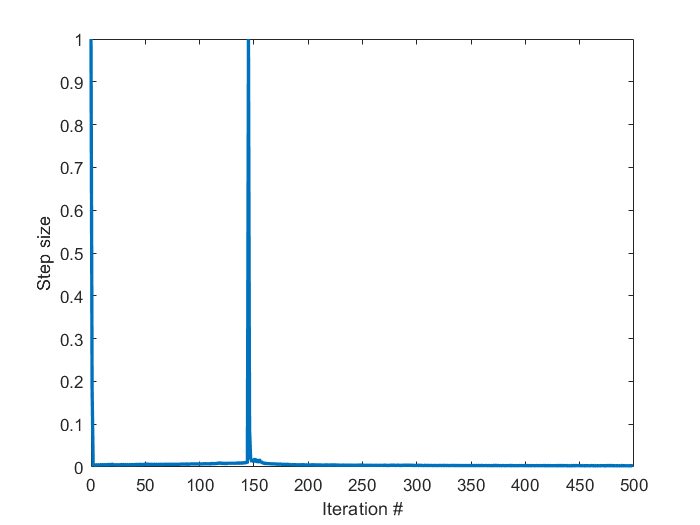
\includegraphics[width=\linewidth]{images/4-1-alpha.png}
                \caption{}
                \label{fig4-1:a}
                \vspace{4ex}
            \end{subfigure}%%
            \begin{subfigure}[b]{0.5\linewidth}
                \centering
                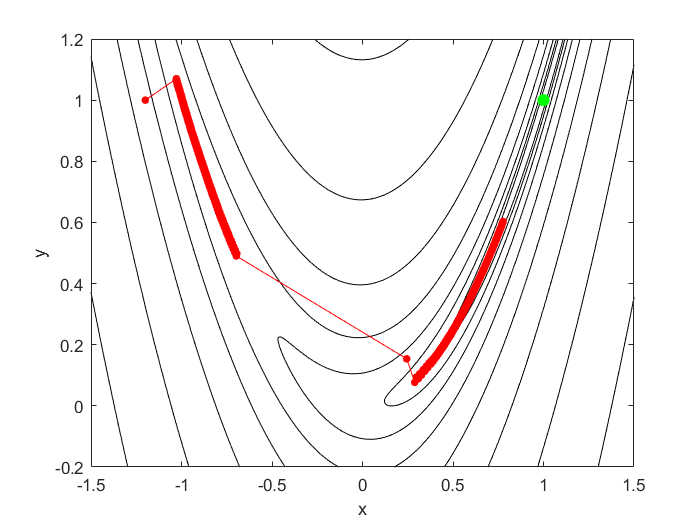
\includegraphics[width=\linewidth]{images/4-1-contour.png}
                \caption{}
                \label{fig4-1:b}
                \vspace{4ex}
            \end{subfigure}
            \caption{For the steepest descent method, the $\alpha_k$ value compared to the $k$th iteration shown in (a) and the iterate (seen in red) plotted on the contour of the Rosenbrock function (seen in black) with the local minimizer $(1,1)$ (seen in green) shown in (b).}
            \label{fig4-1}
        \end{figure}
        \begin{figure}[H]
            \begin{subfigure}[b]{0.5\linewidth}
                \centering
                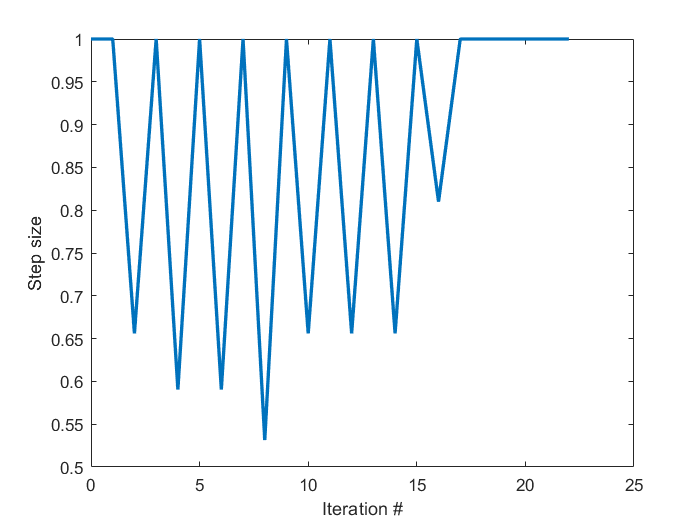
\includegraphics[width=\linewidth]{images/4-2-alpha.png}
                \caption{}
                \label{fig4-2:a}
                \vspace{4ex}
            \end{subfigure}%%
            \begin{subfigure}[b]{0.5\linewidth}
                \centering
                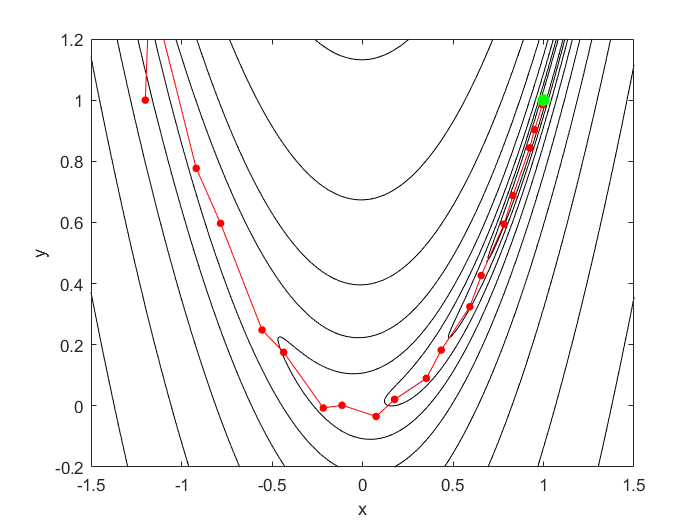
\includegraphics[width=\linewidth]{images/4-2-contour.png}
                \caption{}
                \label{fig4-2:b}
                \vspace{4ex}
            \end{subfigure}
            \caption{For the Newton method, the $\alpha_k$ value compared to the $k$th iteration shown in (a) and the iterate (seen in red) plotted on the contour of the Rosenbrock function (seen in black) with the local minimizer $(1,1)$ (seen in green) shown in (b).}
            \label{fig4-2}
        \end{figure}
        \begin{figure}[H]
        \begin{subfigure}[b]{0.5\linewidth}
            \centering
            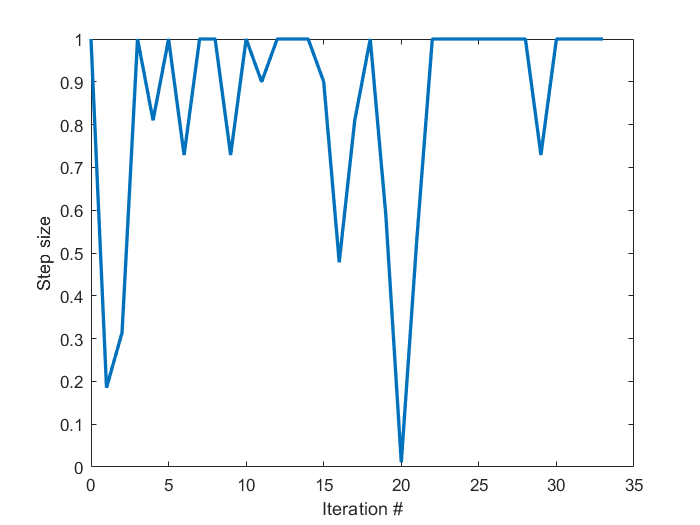
\includegraphics[width=\linewidth]{images/4-3-alpha.png}
            \caption{}
            \label{fig4-3:a}
            \vspace{4ex}
        \end{subfigure}%%
        \begin{subfigure}[b]{0.5\linewidth}
            \centering
            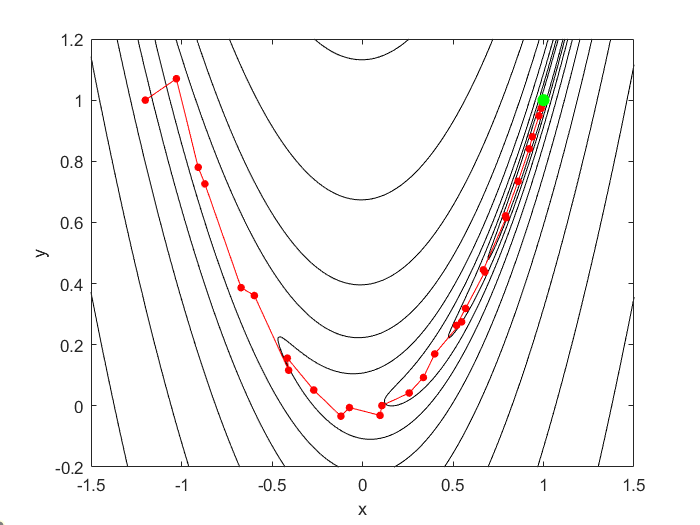
\includegraphics[width=\linewidth]{images/4-3-contour.png}
            \caption{}
            \label{fig4-3:b}
            \vspace{4ex}
        \end{subfigure}
        \caption{For the BFGS method, the $\alpha_k$ value compared to the $k$th iteration shown in (a) and the iterate (seen in red) plotted on the contour of the Rosenbrock function (seen in black) with the local minimizer $(1,1)$ (seen in green) shown in (b).}
        \label{fig4-3}
    \end{figure}
    \begin{figure}[H]
        \begin{subfigure}[b]{0.5\linewidth}
            \centering
            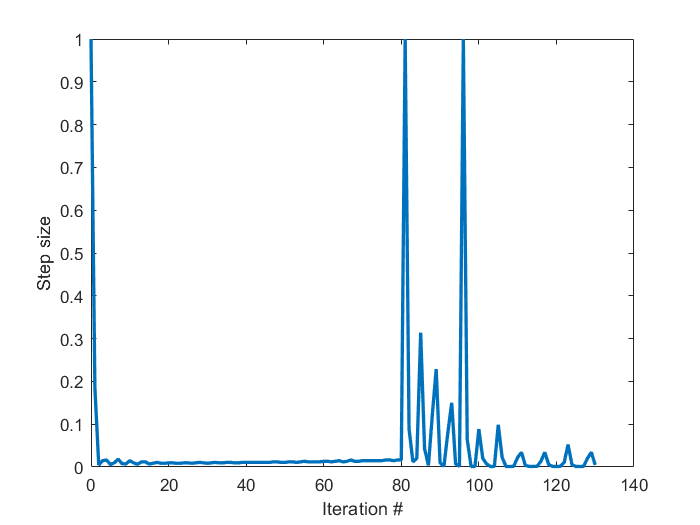
\includegraphics[width=\linewidth]{images/4-4-alpha.png}
            \caption{}
            \label{fig4-4:a}
            \vspace{4ex}
        \end{subfigure}%%
        \begin{subfigure}[b]{0.5\linewidth}
            \centering
            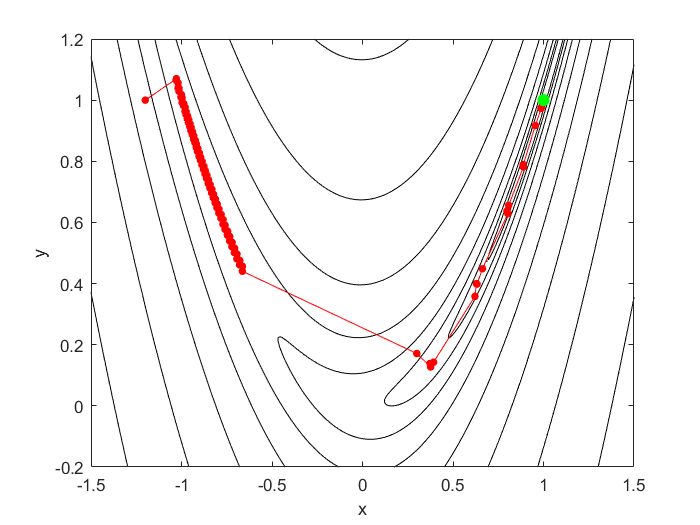
\includegraphics[width=\linewidth]{images/4-4-contour.png}
            \caption{}
            \label{fig4-4:b}
            \vspace{4ex}
        \end{subfigure}
        \caption{For the FRCG method, the $\alpha_k$ value compared to the $k$th iteration shown in (a) and the iterate (seen in red) plotted on the contour of the Rosenbrock function (seen in black) with the local minimizer $(1,1)$ (seen in green) shown in (b).}
        \label{fig4-4}
    \end{figure}
    \begin{figure}[H]
        \begin{subfigure}[b]{0.5\linewidth}
            \centering
            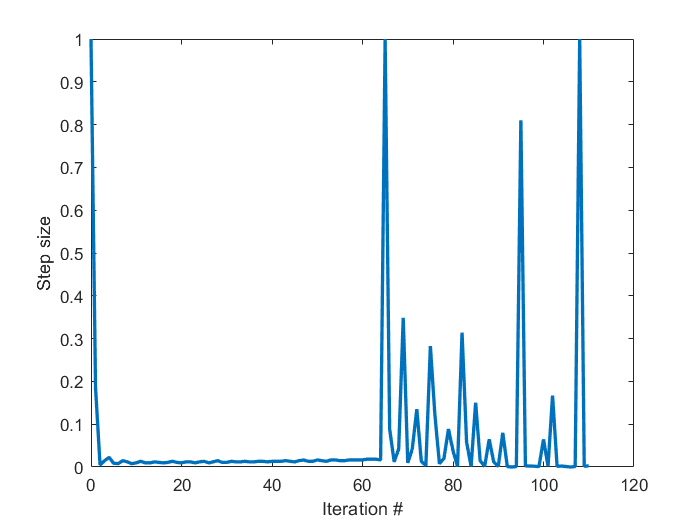
\includegraphics[width=\linewidth]{images/4-5-alpha.png}
            \caption{}
            \label{fig4-5:a}
            \vspace{4ex}
        \end{subfigure}%%
        \begin{subfigure}[b]{0.5\linewidth}
            \centering
            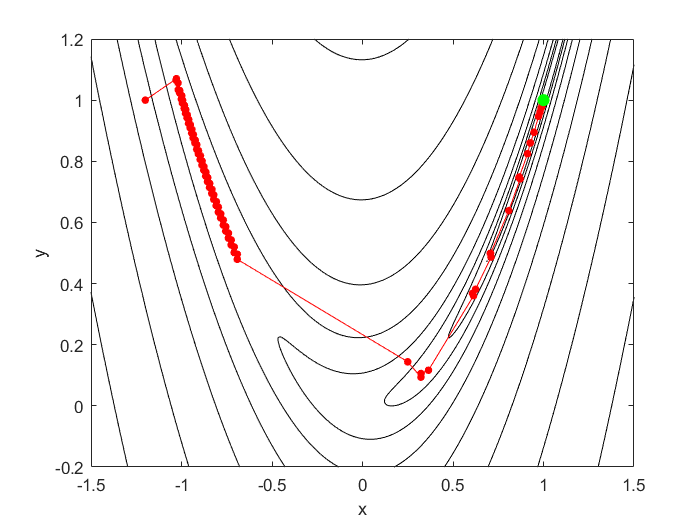
\includegraphics[width=\linewidth]{images/4-5-contour.png}
            \caption{}
            \label{fig4-5:b}
            \vspace{4ex}
        \end{subfigure}
        \caption{For the PRCG method, the $\alpha_k$ value compared to the $k$th iteration shown in (a) and the iterate (seen in red) plotted on the contour of the Rosenbrock function (seen in black) with the local minimizer $(1,1)$ (seen in green) shown in (b).}
        \label{fig4-5}
    \end{figure}
    \begin{figure}[H]
        \centering
        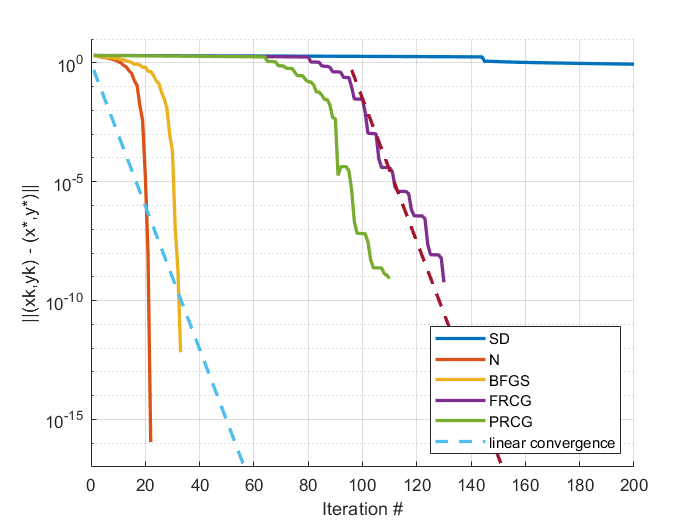
\includegraphics[width=0.8\textwidth,height=\textwidth,keepaspectratio]{images/4-norm.png}
        \caption{The norm $\|(x_k,y_k) - (x^*,y^*)\|$ versus $k$ in the logarithmic scale along the $y$-axis for each method compared to linear convergence (seen in the dotted line).}
        \label{fig4-6}
    \end{figure}

Method created in MatLab:
\begin{lstlisting}[style=Matlab-editor]
function [alphaVals,norms,fvals,xvals,iter] = line_search(func,gfun,Hfun,xstar,x0,dir,print_flag)
    tol = 1e-9; % stop iterations when || grad f|| < tol
    iter_max = 500; % the maximal number of iterations
    BFGSReset = 20;
    % parameters for backtracking line search
    c = 0.45;
    rho = 0.9;
    direction = dir;
    
    x = x0;
    f = func(x);
    g = gfun(x);
    normD = norm(x - xstar);
    %fprintf("Initially, f = %d, ||grad f|| = %d\n",f,norm_g);
    iter = 1;
    
    fvals = zeros(iter_max);
    fvals(1) = f;
    norms = zeros(iter_max);
    norms(1) = normD;
    alphaVals = zeros(iter_max);
    alphaVals(1) = 1;
    xvals = zeros(iter_max,2);
    xvals(1,:) = x;


    fail_flag = 0;
    
    B = eye(length(x));
    while normD > tol && iter < iter_max 
        % choose search direction
        switch direction
            case 1 % steepest descent
                p = -g;
                dir = "SD";
            case 2 % Newton
                H = Hfun(x);
                [~,flag] = chol(H);
                if flag == 0 % H is SPD, use Newton's direction
                    p = -H\g; 
                    dir = "Newton";
                else % use the steepest descent direction
                    p = -g;
                    dir = "SD";
                end
            case 3 % BFGS
                if iter == 1
                    p = -B\g;
                else
                    s = x - xtemp;
                    y = g - gtemp;
                    if(mod(iter,BFGSReset)==0)
                        B = eye(length(x),length(x));
                    else
                        B = B - (B*s*s'*B)/(s'*B*s) + (y*y')/(y'*s);
                    end
                    p = -B\g;
                end
                dir = "BFGS";
            case 4 % Fletcher-Reeves nonlinear CG
                if iter == 1
                    p = - g;
                else 
                    beta = (g'*g)/(gtemp'*gtemp);
                    p = -g + beta *p;
                end 
                dir = "FRCG";
            case 5 % Polak-Ribiere nonlinear CG
                if iter == 1
                    p = -g;
                else
                    beta = (g'*(g-gtemp))/norm(gtemp)^2;
                    beta = max(beta,0);
                    p = -g + beta*p;
                end
                dir = "PRCG";
            otherwise
                return
        end
        % normalize the search direction if its length greater than 1
        norm_p = norm(p);
        if norm_p > 1
            p = p/norm_p;
        end
        % do backtracking line search along the direction p
        a = 1;
        f_temp = func(x + a*p);
        cpg = c*p'*g;
        while f_temp > f + a*cpg % check Wolfe's condition 1
            a = a*rho;
            if a < 1e-14
                fprintf("line search failed\n");
                iter = iter_max;
                fail_flag = 1;
                break;
            end
            f_temp = func(x + a*p);        
        end
        xtemp = x;
        gtemp = g;
        
        x = x + a*p;
        f = func(x);
        g = gfun(x);
        
        normD = norm(x - xstar);
        
        if print_flag == 1
            fprintf("iter %d : dir = %s, f = %d, step length = %d, norm = %d\n",iter,dir,f,a,normD);
        end
        iter = iter + 1;
        fvals(iter) = f;
        norms(iter) = normD;
        alphaVals(iter) = a;
        
        xvals(iter,:) = x;
        if fail_flag == 1
            break;
        end
    end
    fprintf("iter %d : dir = %s, f = %d, step length = %d, norm = %d\n",iter,dir,f,a,normD);
end
\end{lstlisting}
\end{proof}
\end{problem}









\end{document}